\section{Basic architecture}
In this section, we present our approach to implementing the Bitcoin Mining FPGA. We will derive the base architecture of the system from the target algorithm, as well as present the method of internal communication between the components of the system. Finally, the connection to the host will be depicted.

\subsection{SHA-256 Implementation}
For the purposes of work-sharing, modularity, and testing, it is imperative to divide the computation of a SHA-256 hash among different components. While the preprocessing is done in a single component, we split the hash computation into two parts based on the functionality and the data being processed.

\subsubsection*{Padder}
The preprocessing, which consists of the padding, is done in a component appropriately named padder. The output of the padder ($M_0^{(i)},\dots,M_{15}^{(i)}$) is only dependent on the input length, so we hardcode the specific padding logic for both possible input lengths for the SHA-256d calculation. The two possible lengths are 640 bit for the first hash of a block header and 256 bit for the second hash of a SHA-256 hash digest. Furthermore, we implement two different padder components, each specialized on an input size to eliminate the need for any control logic. This, along with known input lengths, allows both padders to be implemented with concurrent statements as in figure~ \ref{code:padder}, making them clock-less, simple, and efficient.

\begin{figure}
    \begin{verbatim}
        padded_message(511 downto 255) <= hash_buffer & '1';
        padded_message(254 downto 9) <= (others => '0');
        padded_message(8 downto 0) <= "100000000";
    \end{verbatim}
    \centering
    \caption[Code of the padder for a 256-bit message]{Code of the padder for a 256-bit message}
    \label{code:padder}
\end{figure}

The padded message is then divided into chunks, which are processed sequentially by the next component, the extender. Each chunk is now interpreted as 16 32-bit words.

\subsubsection*{Extender}

The task of the extender is to generate 64 message schedule words ($W_0,\dots, W_{63}$) from the padded chunk. The first 16 words are directly adopted from the received chunk, while each subsequent word is generated using the preceding 16 words. As we will discuss later, data dependencies allow for two words to be generated concurrently. 

\subsubsection*{Compressor}

The compressor holds the working variables, which get transformed for 64 rounds using message schedule words as specified in the previous section. As each round depends on the previous one, the compressor cannot be parallelized and is thus the main performance-critical part of the system.

To eliminate the need for a large buffer for the message schedule words generated by the extender, we do not precompute them in favor of synchronous calculation while the compressor is running. Furthermore, we already add the constants K\textsubscript{t} to W\textsubscript{t} in the extender prior to passing W\textsubscript{t} to the compressor. This removes the need for the compressor to keep track of the current round number, reducing its complexity.

To compute a Bitcoin block hash, the block header has to be hashed twice. While it is possible to sequentially compute both hash digests on a single set of components, this introduces additional control logic and discourages stage-specific optimizations (e.g. hard-coding the padder for 640 and 256 bits). Therefore we decided to chain two sets of components needed for the computation of SHA-256, as seen in figure~ \ref{fig:mining-core}.

\begin{figure}
    \centering
    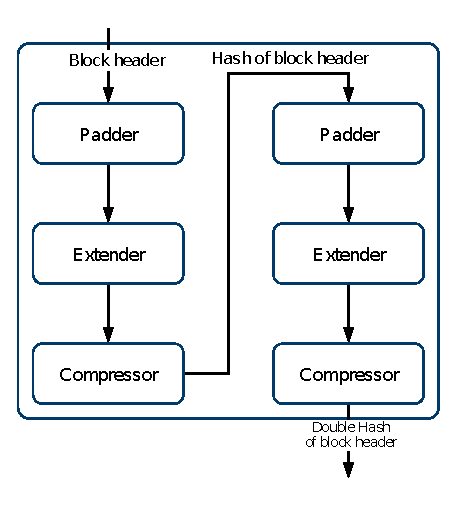
\includegraphics[height=9cm]{img/Mining-core.eps}
    \caption[Components for the computation of a SHA-256d hash]{Components for the computation of a SHA-256d hash}
    \label{fig:mining-core}
\end{figure}
%	- Nonce generator ?? siehe latex.tum.de
% 	- Comparator??

\subsection{Internal Communication}

\label{internal_com}

% Bezieht sich vor allem auf die Komponenten der SHA-256 Implementierung
In order that the padder, extender, and compressor components work together seamlessly, a common communication protocol is required. Such a protocol should include the intermediate hash value calculations as well as additional signals to synchronize the transfer of information.

\subsubsection*{First Approach: Master-Slave Communication Protocol with Feedback}
Our first approach to synchronize the data transfer between the SHA-256 components was to implement a feedback-based master-slave protocol. The master sends a chunk of data to the slave and waits until it confirms that the data chunk has been processed before sending the next one. For this, the master possesses an outgoing "enable" signal to inform the slave about new data. Additionally, the slave component has an outgoing "ready" signal to the master which communicates if it is ready to receive new data. This approach is visualized in figure \ref{Fig:protocol}. The main advantage of this communication protocol is that components don't need to know the execution times of other components and thus are more independent from each other.

\begin{figure}
\centering

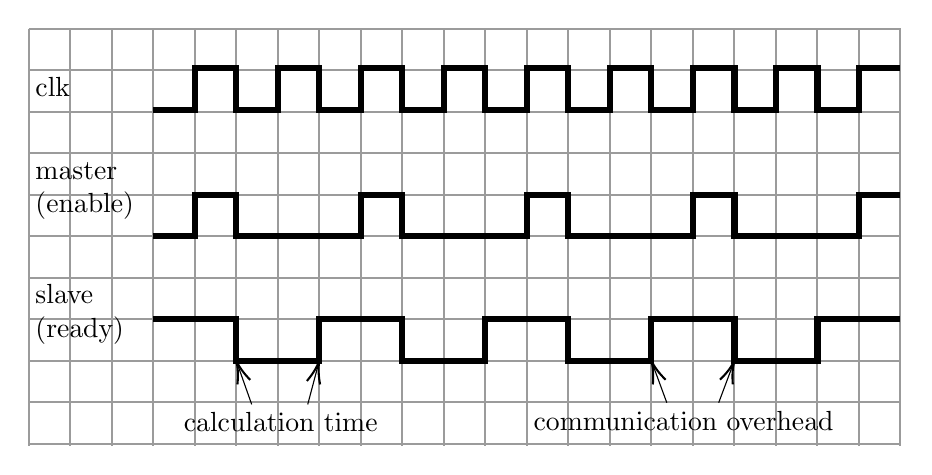
\begin{tikzpicture}[x=0.75pt,y=0.75pt,yscale=-1,xscale=1]
%uncomment if require: \path (0,310); %set diagram left start at 0, and has height of 310

%Shape: Grid [id:dp832068707797099] 
\draw  [draw opacity=0][line width=0.75]  (29.5,59.7) -- (449.93,59.7) -- (449.93,260.7) -- (29.5,260.7) -- cycle ; \draw  [color={rgb, 255:red, 155; green, 155; blue, 155 }  ,draw opacity=1 ][line width=0.75]  (29.5,59.7) -- (29.5,260.7)(49.5,59.7) -- (49.5,260.7)(69.5,59.7) -- (69.5,260.7)(89.5,59.7) -- (89.5,260.7)(109.5,59.7) -- (109.5,260.7)(129.5,59.7) -- (129.5,260.7)(149.5,59.7) -- (149.5,260.7)(169.5,59.7) -- (169.5,260.7)(189.5,59.7) -- (189.5,260.7)(209.5,59.7) -- (209.5,260.7)(229.5,59.7) -- (229.5,260.7)(249.5,59.7) -- (249.5,260.7)(269.5,59.7) -- (269.5,260.7)(289.5,59.7) -- (289.5,260.7)(309.5,59.7) -- (309.5,260.7)(329.5,59.7) -- (329.5,260.7)(349.5,59.7) -- (349.5,260.7)(369.5,59.7) -- (369.5,260.7)(389.5,59.7) -- (389.5,260.7)(409.5,59.7) -- (409.5,260.7)(429.5,59.7) -- (429.5,260.7)(449.5,59.7) -- (449.5,260.7) ; \draw  [color={rgb, 255:red, 155; green, 155; blue, 155 }  ,draw opacity=1 ][line width=0.75]  (29.5,59.7) -- (449.93,59.7)(29.5,79.7) -- (449.93,79.7)(29.5,99.7) -- (449.93,99.7)(29.5,119.7) -- (449.93,119.7)(29.5,139.7) -- (449.93,139.7)(29.5,159.7) -- (449.93,159.7)(29.5,179.7) -- (449.93,179.7)(29.5,199.7) -- (449.93,199.7)(29.5,219.7) -- (449.93,219.7)(29.5,239.7) -- (449.93,239.7)(29.5,259.7) -- (449.93,259.7) ; \draw  [color={rgb, 255:red, 155; green, 155; blue, 155 }  ,draw opacity=1 ][line width=0.75]   ;
%Straight Lines [id:da081269978474381] 
\draw [line width=2.25]    (89.5,98.73) -- (109.5,98.73) -- (109.5,78.73) -- (129.5,78.73) -- (129.5,98.73) -- (149.5,98.73) -- (149.5,78.73) -- (169.5,78.73) -- (169.5,98.73) -- (189.5,98.73) -- (189.5,78.73) -- (209.5,78.73) -- (209.5,98.73) -- (229.5,98.73) -- (229.5,78.73) -- (249.5,78.73) -- (249.5,98.73) -- (269.5,98.73) -- (269.5,78.73) -- (289.5,78.73) -- (289.5,98.73) -- (309.5,98.73) -- (309.5,78.73) -- (329.5,78.73) -- (329.5,98.73) -- (349.5,98.73) -- (349.5,78.73) -- (369.5,78.73) -- (369.5,98.73) -- (389.5,98.73) -- (389.5,78.73) -- (409.5,78.73) -- (409.5,98.73) -- (429.5,98.73) -- (429.5,78.73) -- (449.5,78.73) ;
%Straight Lines [id:da11451899488705086] 
\draw [line width=2.25]    (89.5,159.7) -- (109.5,159.7) -- (109.5,139.7) -- (129.5,139.7) -- (129.5,159.7) -- (189.5,159.7) -- (189.5,139.7) -- (209.5,139.7) -- (209.5,159.7) -- (269.5,159.7) -- (269.5,139.7) -- (289.5,139.7) -- (289.5,159.7) -- (349.5,159.7) -- (349.5,139.7) -- (369.5,139.7) -- (369.5,159.7) -- (429.5,159.7) -- (429.5,139.7) -- (449.5,139.7) ;
%Straight Lines [id:da6880528054054483] 
\draw [line width=2.25]    (89.5,199.7) -- (129.5,199.7) -- (129.5,219.7) -- (169.5,219.7) -- (169.5,199.7) -- (209.5,199.7) -- (209.5,219.7) -- (249.5,219.7) -- (249.5,199.7) -- (289.5,199.7) -- (289.5,219.7) -- (329.5,219.7) -- (329.5,199.7) -- (369.5,199.7) -- (369.5,219.7) -- (409.5,219.7) -- (409.5,199.7) -- (449.5,199.7) ;
%Straight Lines [id:da16227358562423388] 
\draw    (163.93,240.7) -- (168.99,221.63) ;
\draw [shift={(169.5,219.7)}, rotate = 464.85] [color={rgb, 255:red, 0; green, 0; blue, 0 }  ][line width=0.75]    (10.93,-3.29) .. controls (6.95,-1.4) and (3.31,-0.3) .. (0,0) .. controls (3.31,0.3) and (6.95,1.4) .. (10.93,3.29)   ;
%Straight Lines [id:da3772005447416509] 
\draw    (136.93,240.7) -- (130.17,221.59) ;
\draw [shift={(129.5,219.7)}, rotate = 430.51] [color={rgb, 255:red, 0; green, 0; blue, 0 }  ][line width=0.75]    (10.93,-3.29) .. controls (6.95,-1.4) and (3.31,-0.3) .. (0,0) .. controls (3.31,0.3) and (6.95,1.4) .. (10.93,3.29)   ;
%Straight Lines [id:da6747894343106903] 
\draw    (336.93,239.87) -- (330.19,221.58) ;
\draw [shift={(329.5,219.7)}, rotate = 429.77] [color={rgb, 255:red, 0; green, 0; blue, 0 }  ][line width=0.75]    (10.93,-3.29) .. controls (6.95,-1.4) and (3.31,-0.3) .. (0,0) .. controls (3.31,0.3) and (6.95,1.4) .. (10.93,3.29)   ;
%Straight Lines [id:da6720772320038452] 
\draw    (361.93,239.87) -- (368.8,221.57) ;
\draw [shift={(369.5,219.7)}, rotate = 470.57] [color={rgb, 255:red, 0; green, 0; blue, 0 }  ][line width=0.75]    (10.93,-3.29) .. controls (6.95,-1.4) and (3.31,-0.3) .. (0,0) .. controls (3.31,0.3) and (6.95,1.4) .. (10.93,3.29)   ;

% Text Node
\draw (31.5,122.7) node [anchor=north west][inner sep=0.75pt]  [font=\normalsize] [align=left] {master\\(enable)};
% Text Node
\draw (31.5,81.73) node [anchor=north west][inner sep=0.75pt]  [font=\normalsize] [align=left] {clk};
% Text Node
\draw (31.5,181.73) node [anchor=north west][inner sep=0.75pt]  [font=\normalsize] [align=left] {slave\\(ready)};
% Text Node
\draw (103,243.3) node [anchor=north west][inner sep=0.75pt]   [align=left] {calculation time};
% Text Node
\draw (271.5,242.7) node [anchor=north west][inner sep=0.75pt]   [align=left] {communication overhead};


\end{tikzpicture}

\caption{Rising edge clocked master slave communication protocol}
\label{Fig:protocol}
\end{figure}

However, this communication protocol isn't well suited for a speed optimized FPGA design because the duration between setting the ready signal and receiving the next enable signal cannot be used by the child component to perform calculations.

\subsubsection*{Better Approach: Individual Communication Protocol for Each Component}

The most efficient way to reduce the aforementioned communication overhead is to make use of the knowledge about other component's execution times, more specifically the number of clock cycles a master component has to wait before sending the next data to its slave. We'll demonstrate this by taking a closer look at the padder-extender and extender-compressor connections using this improved approach. In general, the bottlenecks of our SHA-256 implementation are the extender and compressor components, as they have to perform internal calculations for each of the 64 rounds. Thus, we will focus on removing the communication overhead in these two components.

As for the padder-extender connection, one can e.g. implement a slightly modified master-slave communication protocol. We already know that the padder only needs one cycle to generate a new padded chunk and that the extender needs considerably more cycles to process it. To let the extender work without a communication overhead, the extender can send the ready signal two cycles before finishing its own calculations. After one cycle, the padder receives the ready signal from the extender and after another clock cycle, the next padded chunk is available for the extender. Consequently, the extender can immediately continue with calculating the next block header.

The extender-compressor connection can be realized through three one-bit signals from the extender to the compressor in addition to the data vector. This allows the extender to notify the compressor about relevant events: when data is sent, when a new block header is processed, and when the last piece of information belonging to the current block header is sent. The compressor doesn't need to give feedback to the extender after calculating a hash because both components have the same duration of execution.

\subsection{External Communication}  
\label{ssec:externalCommunication}

In order to send the data to work on to the FPGA and to receive the result, we need a connection between the FPGA and host.
Due to our very specialized task, the FGPA just has to understand two communication requests:

\begin{enumerate}
	\item Receive a block header.
	\item Send the current nonce and whether it leads to a valid hash digest.
\end{enumerate}

If we look at figure \ref{fig:headerformat}, we can see that all information necessary (header and target) for computing hashes and comparing these against the target value is already included in the header. 
Therefore, no further information has to be sent for the calculation. 
Technically we do not need to pass the nonce, which is the last 32 bits of header, as this value is meant to be changed for each hash. 
For easier testing, however, it is still included and used as the base value that the FPGA begins computing hashes from.
Once a new header is sent, the FGPA is reset and immediately starts with the new calculation.
This is justified because when we send a new header to the FPGA, it is either due to detecting that the previous header would lead to an invalid block or already having found a valid hash for the previous header.
It would then be of no use to further work on it.
One of these situations occurs every time we or another miner found a block which includes some transactions included in the header we are currently computing hashes for.

Upon first inspection, it appears quite obvious that we should return the calculated hash along with the nonce and a bit showing whether the search was successful for the response. 
The problem with this approach is the resource consumption of the logic gathering the hash and sending it back to the host.
Since finding a valid nonce happens quite rarely, this part of the board would be unused most of the time. 
Therefore, we only send back the current nonce and a found bit and opt to calculate the SHA-256d hash on the host for the case where the nonce is valid.

Another point we have to care about is keeping the stall cycles of the FPGA as low as possible. 
That is to say, ensuring the FPGA starts with the next header as soon as possible after finding a valid block or finishing all possible nonces. 
At first some sort of header queue comes to ones mind. However, this would consume resources to store another 640 bit header on the FPGA board and is therefore not optimal.

In our case, there is a much simpler solution, but the following considerations only work based on the assumption that the time for trying all $2^{32}$ nonces is significantly greater than one second. 
For the highest achieved nonce rate of $\maxHashrate$, we need $ 2^{32} \textit{Hash} / \maxHashrate \approx 85.9s \gg 1s$ to try out all different nonces. After all nonces for a given header have been tried out without success, we have to change another part of the header. 
The simplest change that can be done is the increment of the timestamp.
Since the time is represented in UNIX Epoch time, an increment by one represents a time increment by one second. Here our assumption assures that we do not surpass the current real-time and always calculate with valid timestamps\footnote{The Bitcoin network accepts timestamps within 2 hours of the network adjusted time. In the unlikely case that no valid hash is found during this time, the timestamp needs to be updated externally.}.

Both request are sent to the FPGA via a Python script using UART. 
On the FPGA we implemented a dedicated component for accepting requests that acts as an interface to the mining components.

%- Externen Anschluss (CLI)
% 	- Benötigte Befehle 
%   - Nächster Header, wenn abgearbeitet? -> Erhöhung des Timestamp
